
%(BEGIN_QUESTION)
% Copyright 2012, Tony R. Kuphaldt, released under the Creative Commons Attribution License (v 1.0)
% This means you may do almost anything with this work of mine, so long as you give me proper credit

Connect a loop-powered differential pressure transmitter (with HART capability along with analog 4-20 mA output) to a DC voltage source, a 250 ohm resistor, and a diode as shown, using parts supplied by the instructor.  You will need to bring your own multimeter for this experiment, but your instructor will supply the HART communicators.  All electrical connections must be made using a terminal strip (no twisted wires, crimp splices, wire nuts, spring clips, or ``alligator'' clips permitted):

$$\includegraphics[width=15.5cm]{i03877x01.eps}$$

\vskip 10pt

When you have your transmitter powered and functioning, answer the following questions:

\begin{itemize}
\item{} Trace the direction of current through this DC circuit (using conventional flow notation) and identify the polarity of the voltage across each component in accordance with that component's function as either an electrical {\it source} or an electrical {\it load}.
\vskip 10pt
\item{} Demonstrate how to measure the transmitter's output signal three different ways:
\itemitem{} Measuring a voltage drop across the 250 $\Omega$ resistor (1-5 V signal)
\itemitem{} Breaking the circuit to directly measure current with a milliammeter (4-20 mA signal)
\itemitem{} Connecting a milliammeter in parallel with the diode (4-20 mA signal)
\vskip 10pt
\item{} How does an applied pressure (blowing into the plastic tube) to the ``High'' pressure port on the transmitter affect the electrical signal?  How about an applied pressure to the ``Low'' pressure port?
\vskip 10pt
\item{} Explain how the differential pressure transmitter, with its ``High'' and ``Low'' pressure ports, can act either as a {\it direct-acting} or as a {\it reverse-acting} instrument.
\vskip 10pt
\item{} While measuring current (with the milliammeter shorting across the diode), temporarily short past the 250 ohm resistor with a jumper wire.  How does this affect the circuit current, and why?
\vskip 10pt
\item{} Use the data-recording (``Min/Max'') mode of your digital multimeter to capture the highest loop current signal value, as well as the lowest, explaining how this multimeter function might be diagnostically useful.
\vskip 10pt
\item{} Connect a HART communicator device in parallel with the transmitter, turn it on, and use it to access the transmitter's programmable parameters.
\vskip 10pt
\item{} Use a multimeter set to measure {\it AC} volts to detect HART communications in the circuit.  What happens to the AC voltage measurement when the HART communicator is turned off?  Is there any way to capture the peak HART signal values using your multimeter?
\vskip 10pt
\item{} Temporarily short past the resistor with a jumper wire and note whether or not this has any affect on the HART data communications.
\end{itemize}

\vskip 20pt \vbox{\hrule \hbox{\strut \vrule{} {\bf Suggestions for Socratic discussion} \vrule} \hrule}

\begin{itemize}
\item{} How would the pressure transmitter respond if equal pressures were applied to {\it both} ``H'' and ``L'' ports?
\item{} One of the basic rules electronics students learn when first using their multimeters is {\it never} connect an ammeter in {\it parallel} with anything, only in series.  Explain why shorting across the diode is okay to do, and whether or not shorting across the resistor would be just as practical.
\end{itemize}

\underbar{file i03877}
%(END_QUESTION)





%(BEGIN_ANSWER)

Fluke brand multimeters all have a ``Min/Max'' mode useful for recording measurements over long spans of time.  This is an incredibly valuable yet under-utilized diagnostic tool, because it allows the technician to detect certain intermittent conditions by connecting the meter, leaving it alone to record data, then checking later to see whether a particular event occurred in the interim.

%(END_ANSWER)





%(BEGIN_NOTES)

\vskip 20pt \vbox{\hrule \hbox{\strut \vrule{} {\bf Virtual Troubleshooting} \vrule} \hrule}

This question is a good candidate for a ``Virtual Troubleshooting'' exercise.  Presenting the diagram to students, you first imagine in your own mind a particular fault in the system.  Then, you present one or more symptoms of that fault (something noticeable by an operator or other user of the system).  Students then propose various diagnostic tests to perform on this system to identify the nature and location of the fault, as though they were technicians trying to troubleshoot the problem.  Your job is to tell them what the result(s) would be for each of the proposed diagnostic tests, documenting those results where all the students can see.

During and after the exercise, it is good to ask students follow-up questions such as:

\begin{itemize}
\item{} What does the result of the last diagnostic test tell you about the fault?
\item{} Suppose the results of the last diagnostic test were different.  What then would that result tell you about the fault?
\item{} Is the last diagnostic test the best one we could do?
\item{} What would be the ideal order of tests, to diagnose the problem in as few steps as possible?
\end{itemize}


%INDEX% Differential pressure transmitter circuit

%(END_NOTES)


